\subsection{Explicaci\'on del algoritmo}

Para desarrollar el algoritmo de Búsqueda local, necesitamos definir dos cosas. Una es la \"vecindad\" y la otra cual será nuestra solución inicial.

Consideramos que una clique es vecina de otra si difieren exactamente en un nodo, es decir puede tener un nodo más, un nodo menos o uno distinto (con el mismo número de nodos). Si la clique posee un único nodo, sólo se tienen en cuenta los vecinos que tienen un nodo más, porque no podemos sacar (nos quedaríamos sin solución), y para cambiar un nodo lo que hacemos es primero quitar uno, y después poner uno entre todas las posibilidades que en este caso serían todos los nodos, por lo tanto elegiría el nodo de mayor grado, y justamente no buscamos que empiece por ahí.

La solución inicial es un nodo elegido al azar.
En cada iteración creamos la vecindad de la clique de máxima frontera (CMF) hasta el momento, recorremos sus vecinos y en caso de que tenga mayor frontera que la CMF hasta el momento, ésta pasa a ser la nueva CMF.

Otras vecindades que tuvimos en cuenta fueron:
\begin{itemize}
\item Cliques de igual o diferencia de uno en tamaño.
\item La clique de mayor tamaño que contenga a todos los nodos que forman parte de la solución en ese momento. La consideramos junto con la definición de vecindad que terminamos implementando.
\end{itemize}

Las descartamos porque los algoritmos para encontrar estas cliques vecinas implican una complejidad muy alta, y el proceso para hacerlo no resulta tan directo como el que elegimos, que si bien puede llegar a evaluar un gran número de posibilidades, está muy relacionado con el grado de los nodos y cantidad que tengamos en la solución, ya que si agregamos un nodo será uno de la frontera, si sacamos será uno de la solución que teníamos y si intercambia será entre uno de la solución con uno de la frontera.

La solución inicial es elegida al azar porque nos dimos cuenta que si empezábamos por el nodo de mayor grado, el resultado que obteníamos era el mismo que con la heurística constructiva del algoritmo goloso, al menos para la gran mayoría de familias de grafos.

\textbf{Ejemplo del funcionamiento:}

\begin{center}
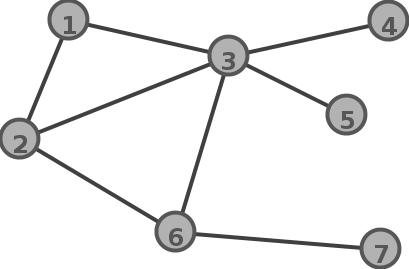
\includegraphics[scale=0.5]{Images/ejemploGrafo.png} 
\end{center}

Dado el siguiente grafo y comenzando por el nodo 4 (elegido al azar) el algoritmo realiza las siguientes iteraciones:
\begin{center}
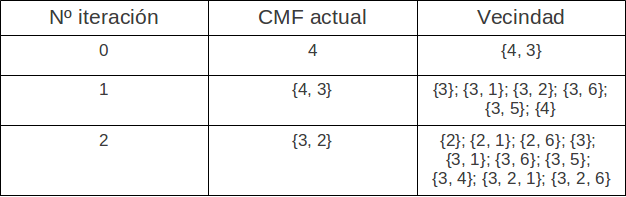
\includegraphics[scale=0.7]{Images/EjemploLocal.png} 
\end{center}

Y el resultado final, que también es el esperado, es: $\lbrace $3, 2$\rbrace$ que tiene una frontera de 6.

\subsection{Pseudoc\'odigo y complejidad}
\begin{algorithm}
	\caption{Busqueda Local}\label{local}
	\begin{algorithmic}[1]
	\Procedure{Local }{$G\ =\ (V,\ E)$}
		\State $CMF=\ random(nodos)$	\Comment{elige un nodo al azar}
		\While{$hay\_ cambio$}			\Comment{si no hay cambios CMF es máx local}
			\State $armar\_ vecindad(CMF)$
			\ForAll{$vecino\ in\ vecindad$}
				\If{$frontera(vecino)\ >\ frontera(CMF)$}
					\State $CMF=\ vecino$
				\EndIf
			\EndFor
		\EndWhile
	\EndProcedure
	\State

	\Procedure{armar\_vecindad}{$Clique\ =\ (V,\ E)$}
		\If{$|V|\ >\ 1$}
			\ForAll{$nodo\ in\ V$}
				\State $vecindad\_agregar(Clique-nodo)$
\Comment{Cliques vecinas con un nodo menos}
				\ForAll{$nodo\_candidato\ in\ nodos\_candidatos(Clique-nodo)$}
					\State $vecindad\_agregar(Clique-nodo+nodo\_candidato)$
\Comment{Cliques vecinas con un nodo intercambiado}
				\EndFor
			\EndFor
		\EndIf
		\ForAll{$nodo\_candidato\ in\ nodos\_candidatos(Clique)$}
			\State $vecindad\_agregar(Clique+nodo\_candidato)$
\Comment{Cliques vecinas con un nodo más}
		\EndFor
	\EndProcedure
\end{algorithmic}
\end{algorithm}

nodos\_candidatos(Clique): retorna un vector con los nodos de G que se pueden agregar a la Clique de forma que esta siga siendo un grafo completo.

\textbf{Complejidad: }

La función nodos\_candidatos debe recorrer los nodos de la clique y calcular la intersección entre todos los adyacentes de estos. Por lo tanto una cota holgada para esta función sería O($n^3$). 
Holgada porque si hay n nodos en la clique, no hay más nodos para agregar, por lo tanto la intersección entre los dos primeros sería vacío y no tiene porque continuar.

Luego, la función armar\_vecindad recorre los nodos de la clique (linea 15), llama a nodos\_candidatos dos veces (lineas 17 y 22) y los recorre una vez (linea 22). 
La cantidad de nodos de la clique es a lo sumo n y los nodos candidatos también. Entonces su complejidad es: O(n)*O(n\^{3}) + O(n) = O($n^4$).

Por último la función local, llama a armar\_vecindad (linea 4) y recorre la vecindad (linea 5) una vez por iteración, mientras haya cambio.

El tamaño de la vecindad está dado por la siguiente cuenta, en una clique de k nodos:

\begin{center}
\begin{tabular}{  c  c  }
(vecinos que tienen un nodo menos) & k elecciones
\\ + & + \\ 
(vecinos que tienen un nodo intercambiado) & k*(n-k) elecciones
\\ + & + \\ 
(vecinos que tienen un nodo más) & (n-k) elecciones
\\ = & = \\
(cantidad de vecinos) & k + k*(n-k) + (n-k)
\end{tabular}
\end{center}

Si buscamos un k de forma que se maximize esa cuenta nos daremos cuenta que k=$n/2$ es el que sirve. Dejando así como máximo tamaño de la vecindad $(n^2/4) +n$. Es decir, recorrer la vecindad es O($n^2$).

Falta ver cuántas veces itera, es decir, cuando deja de haber cambio. En el peor de los casos, la frontera de mi clique va aumentando de a uno, entonces como mucho puede iterar cantidad de aristas (m) de veces.

Cuenta final= cantidad de iteraciones * (armar\_vecindad + recorrerla) = O(m) * (O($n^4$) + O($n^2$)) = O(m*$n^4$)

\subsection{Casos nefastos}


\subsection{Experimentaci\'on}




